% !TeX root = main.tex

\chapter{Back Propagation Through Time}
L'algorithme BPTT appliqué à un réseau neuronal récurrent a pour particularité
de déplier le temps dans l'espace; par exemple, pour apprendre un mot de cinq
caractères, on va créer cinq réseaux non-récurrents qui représentent chaqun un
"temps", soit une lettre de la séquence.

\medskip

Cet algorithme a pour avantage, par rapport à celui RTRL, d'avoir une
complexité temporelle inférieure.

\section{Théorie}

\begin{figure}[!ht]
\begin{center}
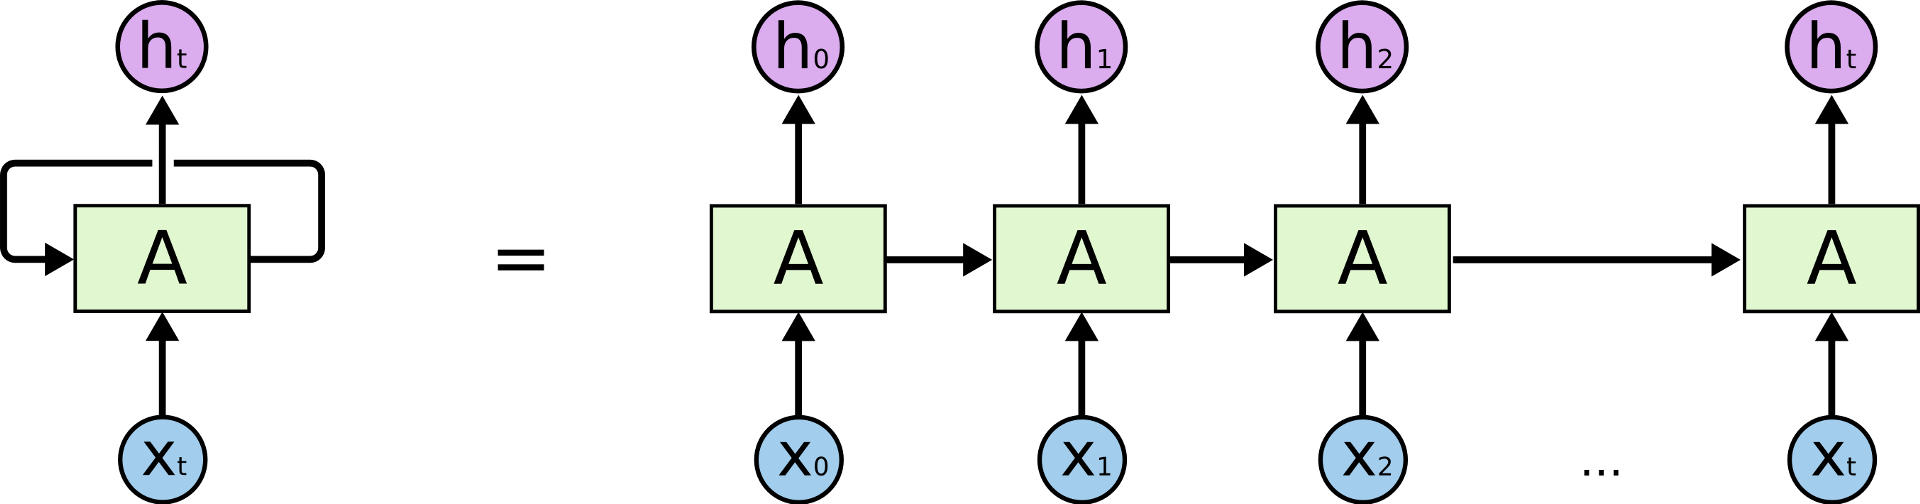
\includegraphics[width=0.8\textwidth]{images/bptt.png}
\caption{Dépliement du temps dans l'espace pour BPTT}
% TODO : crédits
\end{center}
\end{figure}


\subsection{Réseau BPTT}

\section{Implémentation}

L'implémenation est effectuée en C++ via la librairie de calcul matriciel
Eigen3. Toutes les matrices sont des objets de type Eigen::MatrixXd (matrice de
double) et les vecteurs des objets de type Eigen::VectorXd.

\medskip

L'aléatoire utilisé est celui natif en C et C++ : rand.
La génération de la graine se fait à partir du temps à la milliseconde pour
éviter une initialisation déterministe dans le cas de l'execution de plusieurs
runs consécutifs. Pour cela la librairie 'sys/time.h' est utilisée, avec un
appel propre aux systèmes UNIX.

\bigskip

\subsection{Structure de données}

Le code se décompose en plusieurs éléments :
\begin{itemize}
  \item Les poids
  \item Une couche de neurones fully-connected
  \item Le réseau de couches dépliées dans le temps
\end{itemize}

\subsubsection{Les poids}

La classe poids est principalement constituée d'une matrice de poids (carée, de
taille le nombre de neurones). Y est associée une matrice de vartiation de poids
dans laquelle sont stockées toutes les varaitions de poids avant d'être
appliquées. Enfin, il existe un vecteur de biais \verb+bias+ et son vecteur
de variation \verb+delta_bias+ associé.

Enfin, les méthodes de l'objet Poids sont le constructeur et
l'application des variations de poids (qui remet par la même occasion à 0
les delta-poids).

\subsubsection{La couche de neurones}

La couche de neurones (fully-connected) est l'objet élémentaire du réseau. Elle
représente la réseau à un instant t. Elle est crée lors de la propagation d'un
vecteur en entrée à l'instant t et prend en argument un pointeur vers un objet
de type Poids ainsi que ses dimentions.

\medskip

Elle dispose des methodes nécessaires à la propagation et la rétropropagation
d'une entrée à travers le réseau à une couche, stocke ses entrées et sorties
pour les réutiliser lors de la rétropropagation. Lors de la propagation, elle
prend en entrée un vecteur d'entrées et renvoie un vecteur des sorties de
ses neurones. De même, lors de la rétropropagation elle prend en entrée un
vecteur de gradient et en renvoie un autre en sortie. Lors de la
rétropropagation elle calcule aussi les variations de poids à appliquer et les
ajoute au \verb+delta_weight+ de son objet Poids.

\medskip

La fonction d'activation choisie est la sigmoide, la fonction de composition
est la somme, et la fonction de coût est la moitié du coût quadratique (pour
pouvoir dériver plus rapidement).

\medskip

Les attributs de la couche de neurones sont donc les suivants :

\begin{itemize}
  \item \verb+Weights* weights+ l'objet poids qui sera utilisé pour calculer
    les sorties de chaque noeud ;
  \item \verb+Eigen::VectorXd input+ vecteur des entrées de la couche à
    l'instant $t$ ;
  \item \verb+Eigen::VectorXd previous\_output+ vecteur des sorties de la
    couche à l'instant $t-1$ ;
  \item \verb+Eigen::VectorXd output+ sortie de la couche à l'instant $t$.
\end{itemize}

Les méthodes sont donc les suivantes :

\begin{itemize}
  \item \verb+compute( Eigen::VectorXd previous\_output, Eigen::VectorXd input)+
    la methode qui calcule la sortie de la couche. Renvoie \verb+output+ ;
  \item \verb+compute\_gradient(Eigen::VectorXd deltas, Eigen::VectorXd previous\_delta)+
    la methode qui calcule le gradient en entrée de la couche en fonction du
    gradient en sortie. Renvoie \verb+delta\_input+.
\end{itemize}


\subsubsection{Le réseau}

% TODO : détailler fonction, attributs, methodes

\section{Résultats}
Ci-dessous des représentations de l'apprentissage au cours du temps du réseau sur des
grammaires de Reber, simple et double.

\smallskip

En abscisse, le nombre de mots appris, en ordonnée le taux de réussite, testé à
intervalles réguliers sur un échantillon de données de test choisies aléatoirement
dans l'ensemble de test. La zone grise correspond à l'intervalle de confiance à
$95\%$ sur le nombre d'exécutions précisé.

\smallskip

Le réseau utilisé est composé d'une couche cachée de 30 neurones, avec un learning
rate de $0.1$.

\subsection{Grammaire de Reber simple}
Pour une grammaire de Reber simple, la réussite est déterminée par la prédiction
correcte de toutes les transitions des mots testés.

\medskip

Les tests ont été réalisés en apprentissage stochastique (mot par mot) et en
évaluant sur 10000 mots d'un ensemble de test. L'évaluation du taux de réussite
est effectuée tous les 100 mots appris. La fonction de score sélectionée renvoie
1 si toutes les transitions d'un mot ont été prédites, 0 si au moins une des
lettre n'a pas été prédite. Le score total est ensuite rapporté au nombre de
mots testés pour obtenir un taux de réussite.


\begin{figure}[!ht]
\begin{center}
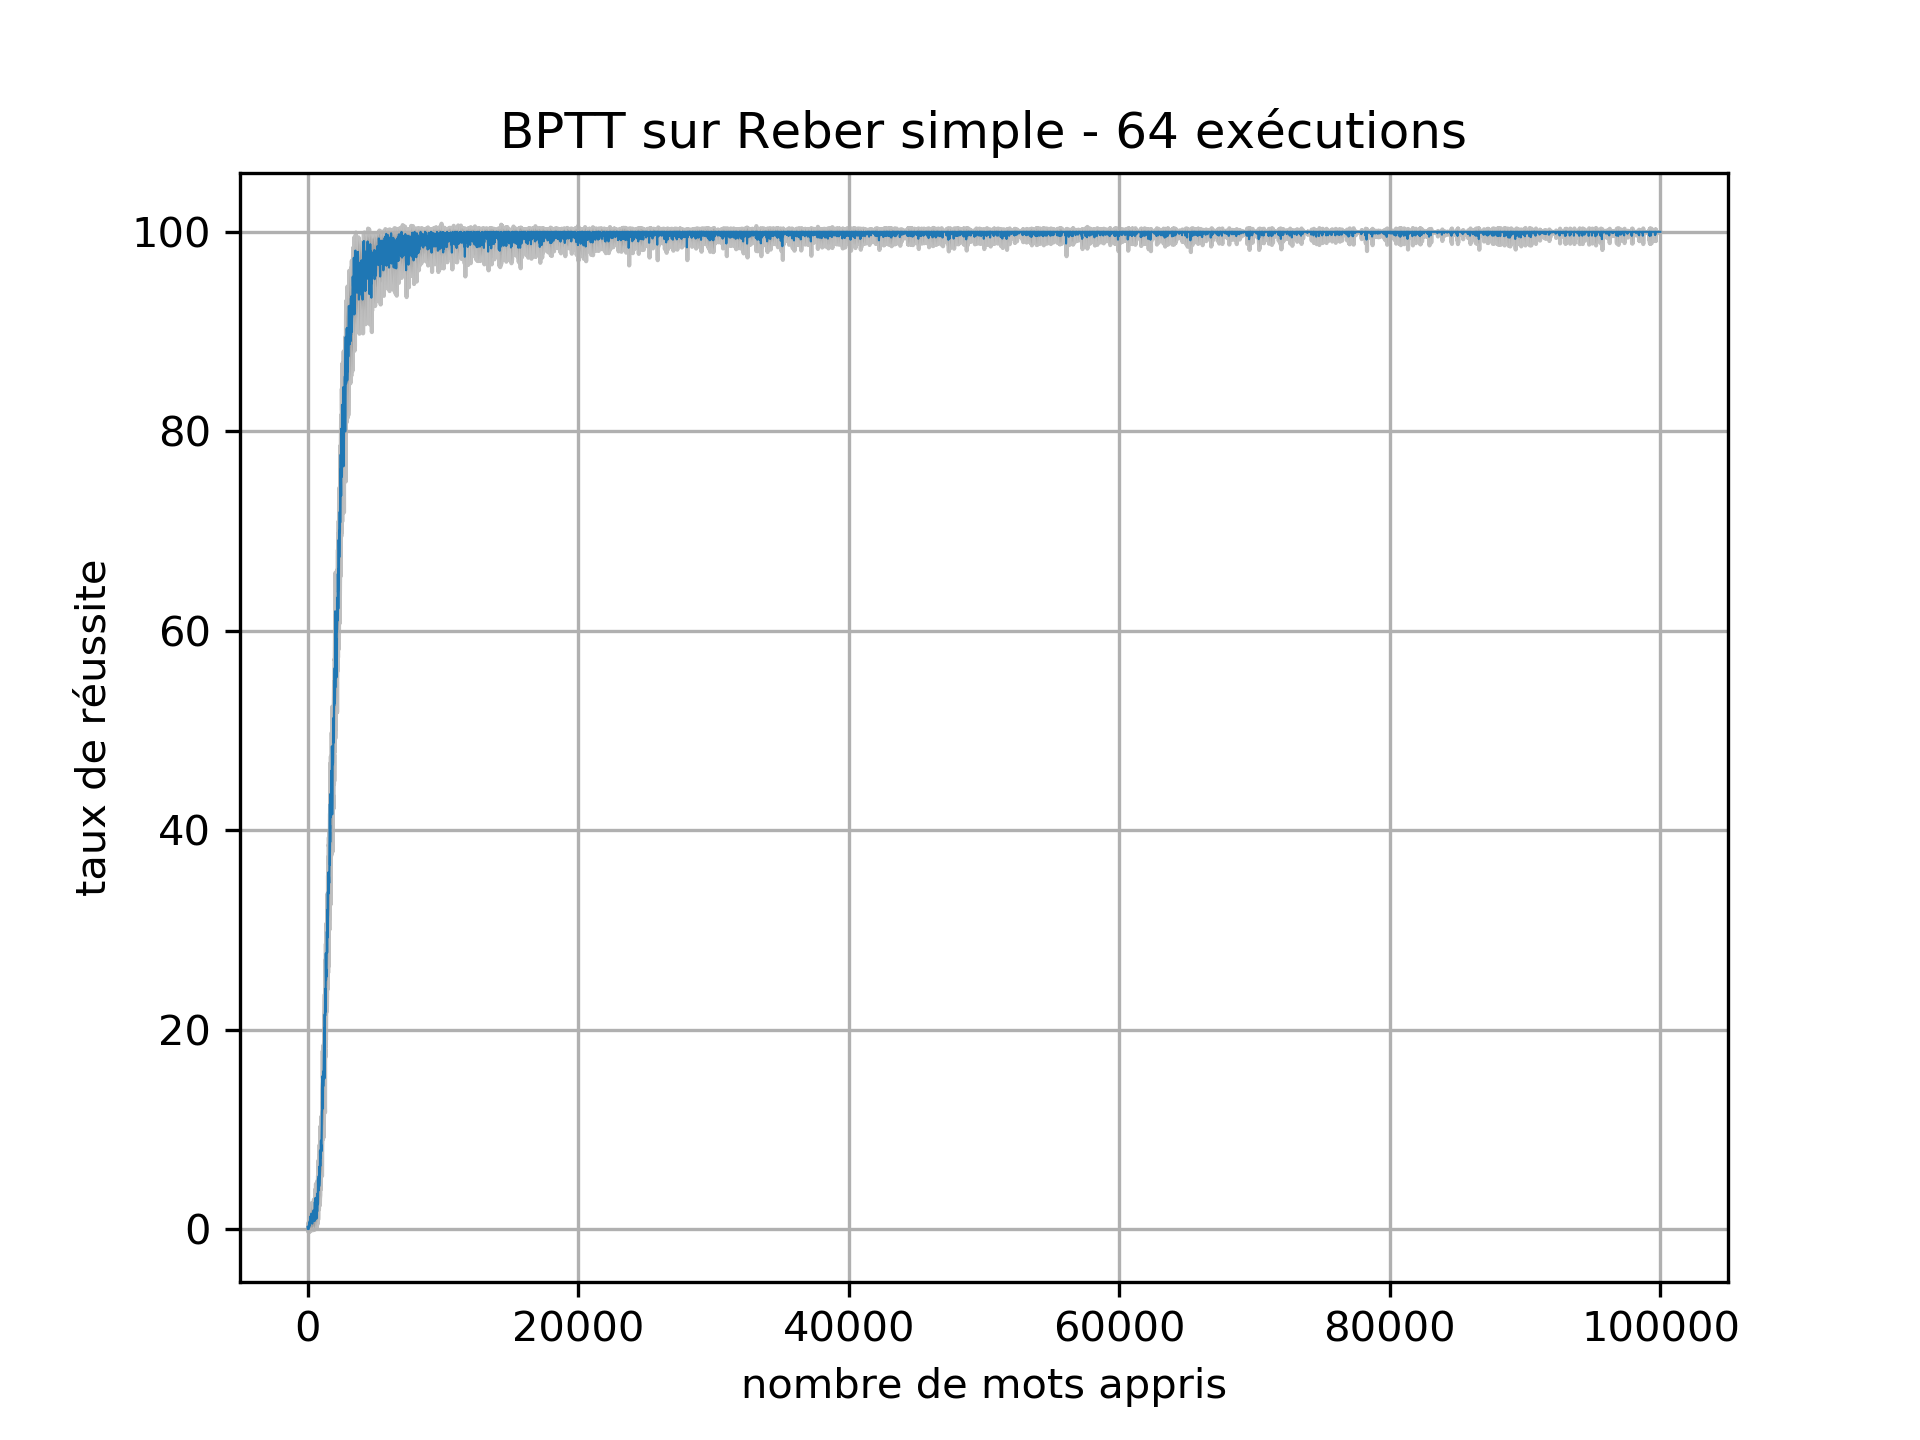
\includegraphics[width=0.7\textwidth]{images/results/bptt_simplereber_ls30_lr01.png}
\caption{Apprentissage au cours du temps, BPTT sur grammaire de Reber simple}
\end{center}
\end{figure}

\medskip

On constate que le réseau apprend de manière certaine la grammaire simple : 
le taux de réussite converge très rapidement vers 100\% et l'écart type
se réduit pour ne plus valoir que 4\%.

\medskip

On peut donc conclure sur la capactité d'un réseau récurrent sur lequel on
applique l'algorithme de mise à jour des poids BPTT à apprendre et prédire les
transitions d'un gramaire de Reber simple ?

\subsection{Grammaire de Reber symétrique}
Pour une grammaire de Reber symétrique, réussite est déterminée par la prédiction
correcte de la première et la dernière transition des mots.

\medskip

Les tests ont été réalisés dans les mêmes conditions que celles de la grammaire
simple. A été évaluée la prediction du dernier carractère en fontion du premier
de la séquence. Les caractères intermédiaires n'ont pas fait l'objet de cette
expérience.

\begin{figure}[!ht]
\begin{center}
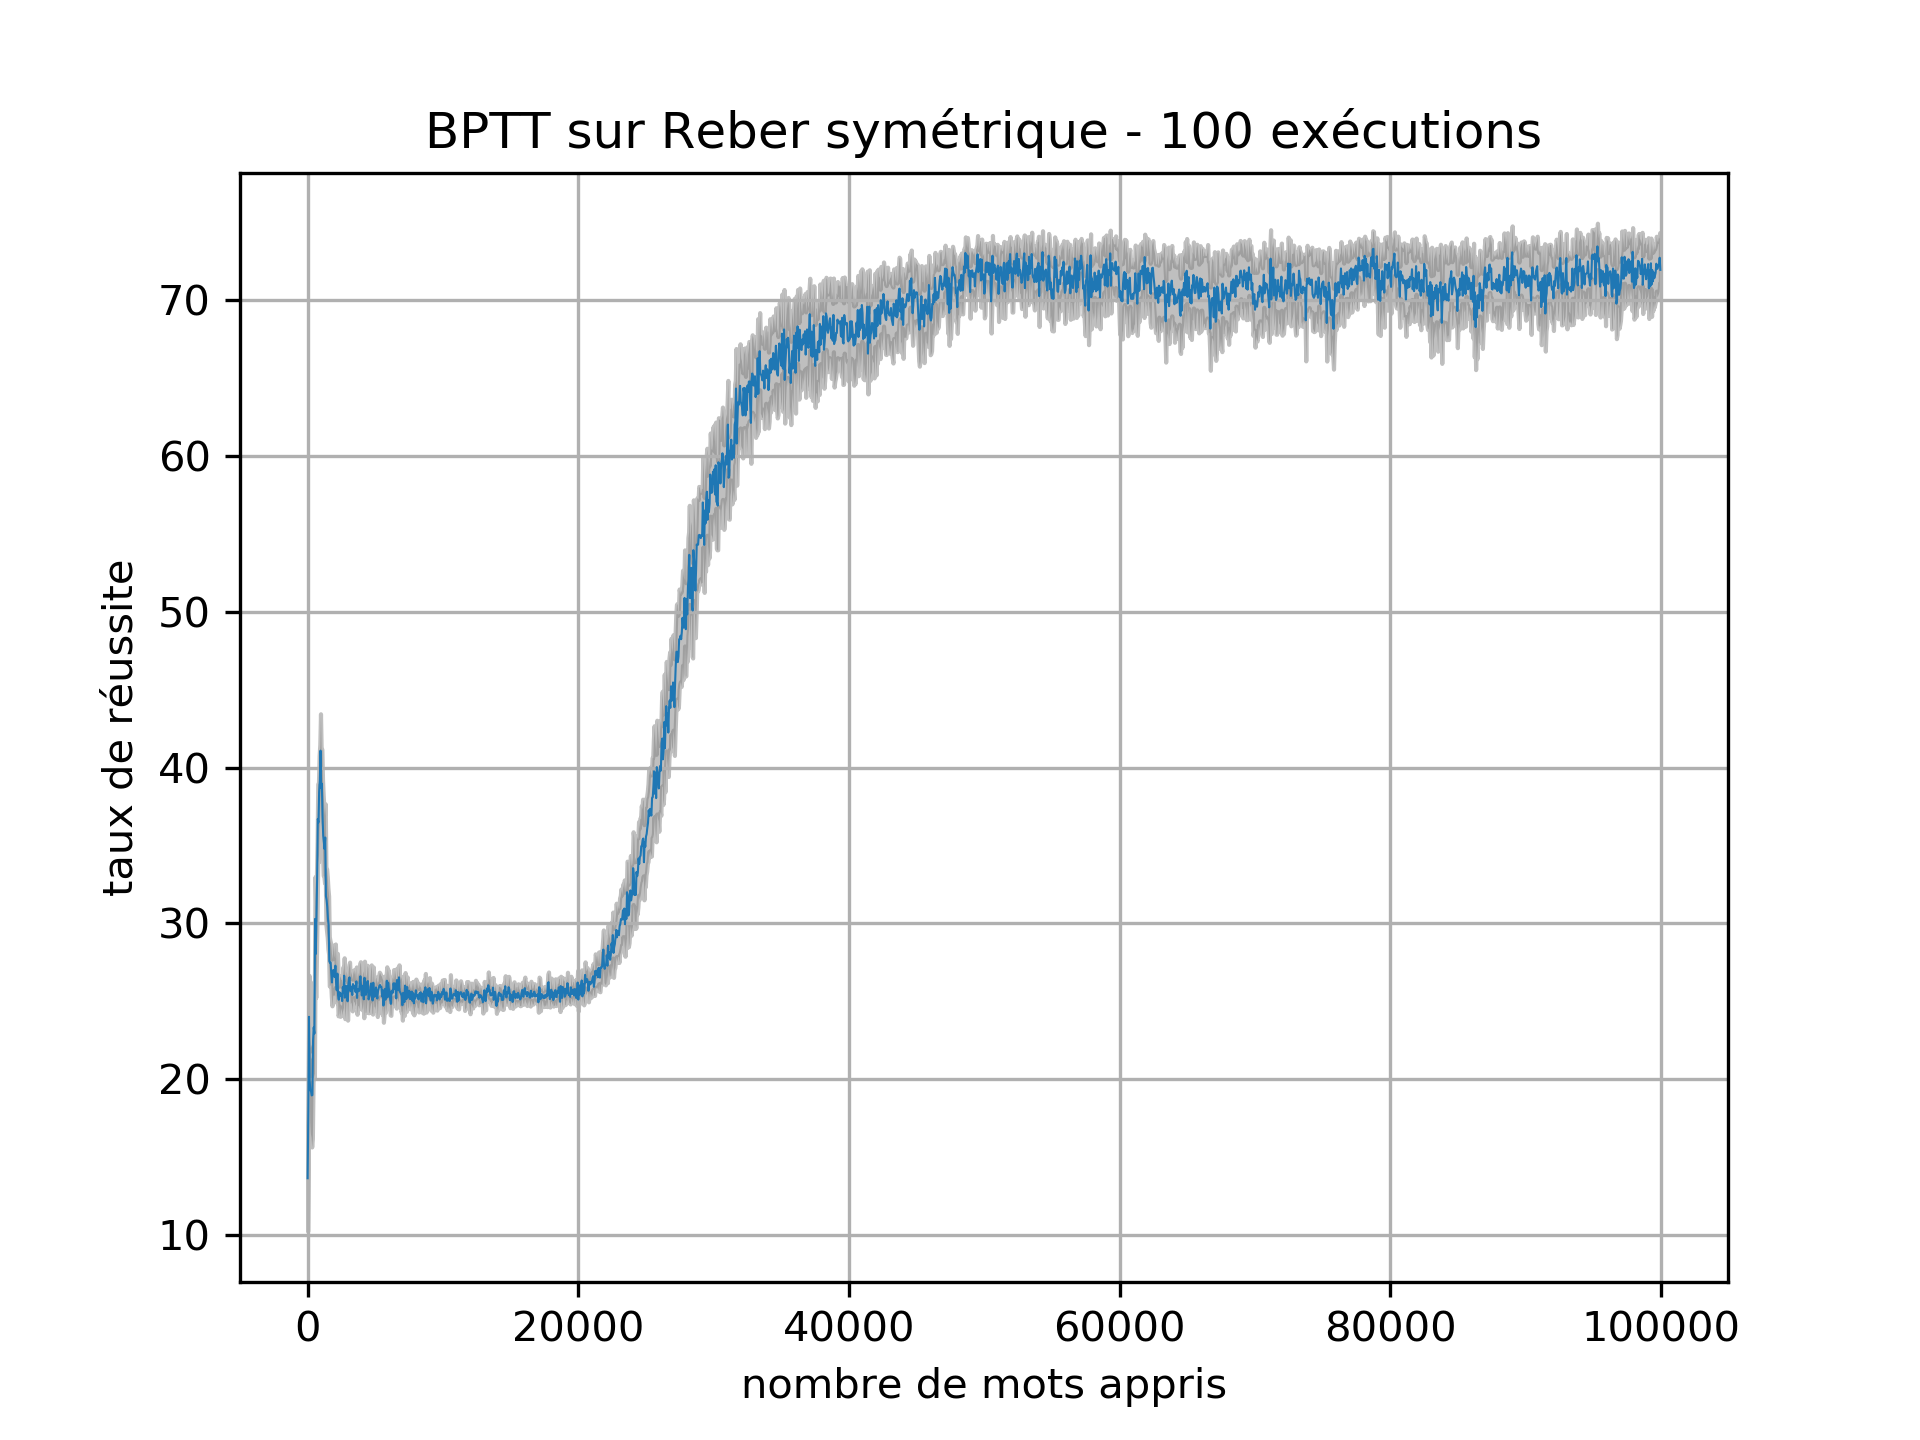
\includegraphics[width=0.7\textwidth]{images/results/bptt_doublereber_ls30_lr01.png}
\caption{Apprentissage au cours du temps, BPTT sur grammaire de Reber symétrique}
\end{center}
\end{figure}

\medskip

On constate que le réseau a plus de difficultés à prédire la dernière lettre de
la séquence. En effet, la valeur finale se situe aux alentours de 75\% de
réussite, l'éacrt type reste constant, et la convergence vers la valeur finale
s'effectue entre 20000 et 50000 mots.
